%%%%%%%%%%%%%%%%%%%%%%%%%%%%%%%%%%%%

\section{線形回帰の推測}

%%%%%%%%%%%%%%%%%%%%%%%%%%%%%%%%%%%%

\subsection{ソフトウェアの回帰出力の読み方}

%%%%%%%%%%%%%%%%%%%%%%%%%%%%%%%%%%%

\begin{frame}
\frametitle{遺伝か環境か？}

{\small 1966年、Cyril Burtは「知能の差異の遺伝的決定：一緒に育てられた双子と別々に育てられた双子の研究」という論文を発表した。データは、一卵性双生児27組（代表的な無作為標本と仮定）のIQスコアで構成されており、一方は養親に、もう一方は実の親に育てられた。}

\begin{center}
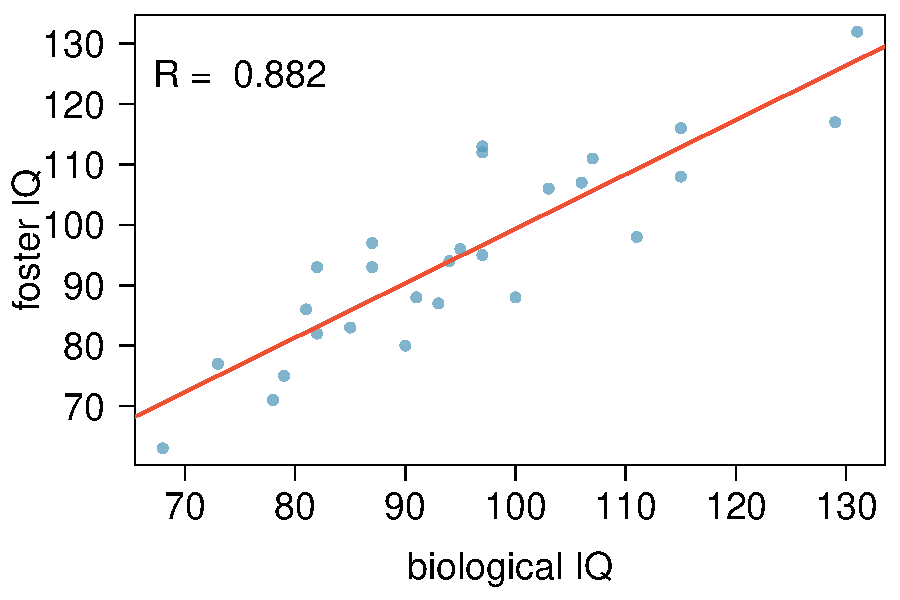
\includegraphics[width=0.7\textwidth]{8-4_inf_lin_reg/figures/twins/twins_IQ}
\end{center}

\end{frame}

%%%%%%%%%%%%%%%%%%%%%%%%%%%%%%%%%%%

\begin{frame}[fragile]
\frametitle{}

\pq{次のうち\underline{誤っている}記述はどれか？}

{\footnotesize
\begin{verbatim}
Coefficients:
                 Estimate Std. Error t value Pr(>|t|)
(Intercept)       9.20760    9.29990   0.990    0.332
bioIQ             0.90144    0.09633   9.358  1.2e-09

Residual standard error: 7.729 on 25 degrees of freedom
Multiple R-squared: 0.7779,	Adjusted R-squared: 0.769
F-statistic: 87.56 on 1 and 25 DF,  p-value: 1.204e-09
\end{verbatim}
}

\begin{enumerate}[(a)]
\item 実の親に育てられた双子のIQが10ポイント高い場合、養親に育てられた双子のIQは平均的に9ポイント高いと関連づけられる。
\solnMult{養親に育てられた双子のIQの約78\%はモデルで正確に予測できる。}
\item 線形モデルは$\widehat{fosterIQ} = 9.2 + 0.9 \times bioIQ$である。
\item 平均より高いIQを持つ養育双子は、平均より高いIQを持つ実親双子と対応している傾向がある。
\end{enumerate}

\end{frame}

%%%%%%%%%%%%%%%%%%%%%%%%%%%%%%%%%%%

\begin{frame}
\frametitle{傾きの検定}

\pq{出生時に引き離されたすべての双子の代表的な標本としてこの27組を想定した場合、実の親に育てられた双子のIQが養親に育てられた双子のIQの有意な予測因子であるかどうかを検定するための適切な仮説はどれか？}

\begin{enumerate}[(a)]
\item \mathhl{H_0:} $b_0 = 0$; \mathhl{H_A:} $b_0 \ne 0$
\item \mathhl{H_0:} $\beta_0 = 0$; \mathhl{H_A:} $\beta_0 \ne 0$
\item \mathhl{H_0:} $b_1 = 0$; \mathhl{H_A:} $b_1 \ne 0$
\solnMult{\mathhl{H_0:} $\beta_1 = 0$; \mathhl{H_A:} $\beta_1 \ne 0$}
\end{enumerate}

\end{frame}

%%%%%%%%%%%%%%%%%%%%%%%%%%%%%%%%%%%

\begin{frame}
\frametitle{傾きの検定（続き）}

{\footnotesize
\begin{center}
\begin{tabular}{rrrrr}
  \hline
 & Estimate & Std. Error & t value & Pr($>$$|$t$|$) \\
  \hline
(Intercept) & 9.2076 & 9.2999 & 0.99 & 0.3316 \\
  bioIQ & 0.9014 & 0.0963 & 9.36 & 0.0000 \\
   \hline
\end{tabular}
\end{center}
}

\begin{itemize}

\item 回帰の推測では常に$t$検定を用いる。$\:$ \\

\Remember{検定統計量 $T = \frac{\text{点推定量} - \text{帰無値}}{SE}$}

\item 点推定量 = $b_1$は観測された傾きである。

\item $SE_{b_1}$は傾きに関連する標準誤差である。

\item 傾きに関連する自由度は$df = n - 2$であり、$n$は標本サイズである。$\:$ \\
\Remember{推定するパラメータ1つにつき自由度を1つ失う。単回帰では$\beta_0$と$\beta_1$の2つのパラメータを推定するため、$df = n - 2$となる。}

\end{itemize}

\end{frame}

%%%%%%%%%%%%%%%%%%%%%%%%%%%%%%%%%%%

\begin{frame}
\frametitle{傾きの検定（続き）}

{\small
\begin{center}
\begin{tabular}{rrrrr}
  \hline
 & Estimate & Std. Error & t value & Pr($>$$|$t$|$) \\
  \hline
(Intercept) &  9.2076 & 9.2999 & 0.99 & 0.3316 \\
  bioIQ & \orange{0.9014}  &   \green{0.0963} & \orange{9.36} & \textcolor{blue}{0.0000} \\
   \hline
\end{tabular}
\end{center}
}

\begin{eqnarray*}
T &=& \frac{\orange{0.9014} - 0}{\green{0.0963}} = \orange{9.36} \\
df &=& 27 - 2 = 25 \\
p\text{値} &=& P(|T| > \orange{9.36}) < \textcolor{blue}{0.01}
\end{eqnarray*}

\end{frame}

%%%%%%%%%%%%%%%%%%%%%%%%%%%%%%%%%%%

\begin{frame}
\frametitle{LA地区における大学卒業率とヒスパニック系住民割合}

\dq{LAの100の郵便番号地域の標本において、大学卒業率とヒスパニック系住民割合の関係について何が言えるか？}

\begin{center}
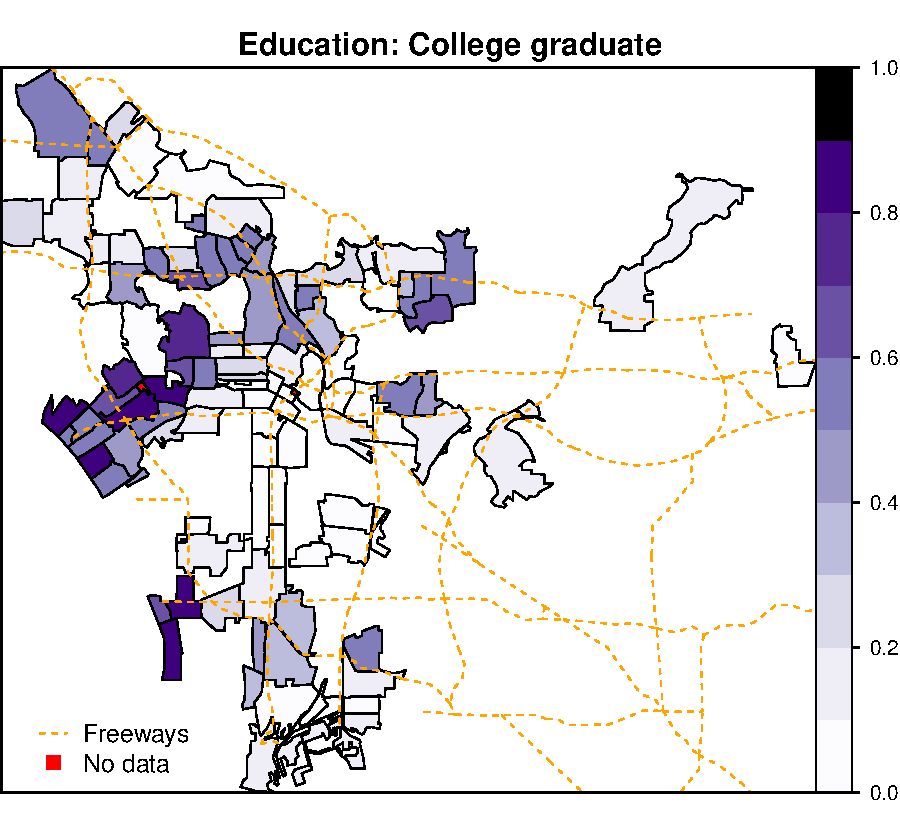
\includegraphics[width=0.46\textwidth]{8-4_inf_lin_reg/figures/la/Prop_EduHigherThan16th}~~~~
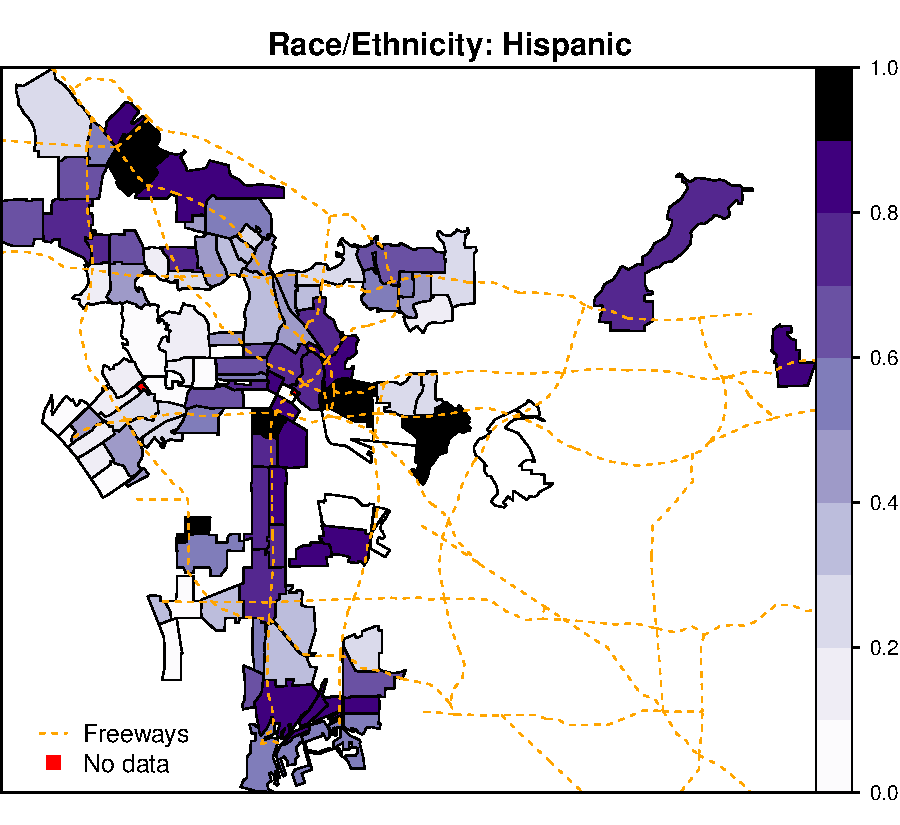
\includegraphics[width=0.46\textwidth]{8-4_inf_lin_reg/figures/la/Prop_RaceEthHispanic}
\end{center}

\end{frame}

%%%%%%%%%%%%%%%%%%%%%%%%%%%%%%%%%%%

\begin{frame}
\frametitle{LA地区における大学卒業率とヒスパニック系住民割合（別の視点）}

\dq{LAの100の郵便番号地域の標本において、大学卒業率とヒスパニック系住民割合の関係について何が言えるか？}

\begin{center}
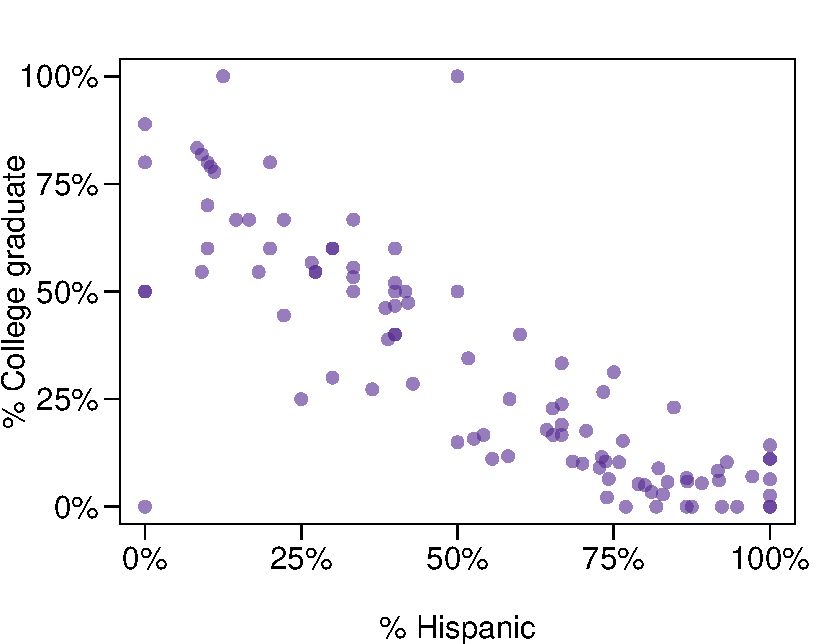
\includegraphics[width=0.7\textwidth]{8-4_inf_lin_reg/figures/la/la}
\end{center}

\end{frame}

%%%%%%%%%%%%%%%%%%%%%%%%%%%%%%%%%%%

\begin{frame}
\frametitle{LA地区における大学卒業率とヒスパニック系住民割合：線形モデル}

\pq{傾きの最もよい解釈はどれか？}

{\small
\begin{center}
\begin{tabular}{rrrrr}
  \hline
 & Estimate & Std. Error & t value & Pr($>$$|$t$|$) \\
  \hline
(Intercept) & 0.7290 & 0.0308 & 23.68 & 0.0000 \\
 \%Hispanic & -0.7527 & 0.0501 & -15.01 & 0.0000 \\
   \hline
\end{tabular}
\end{center}
}

\begin{enumerate}[(a)]
\item LA地区の郵便番号地域でヒスパニック系住民が1\%増加すると、大学卒業率は75\%低下する。
\solnMult{LA地区の郵便番号地域でヒスパニック系住民が1\%増加すると、大学卒業率は0.75\%低下する。}
\item ヒスパニック系住民が1\%追加されるごとに、LA地区の郵便番号地域の大学卒業率は0.75\%低下する。
\item ヒスパニック系住民がいない郵便番号地域では、大学卒業率は75\%と予測される。
\end{enumerate}

\end{frame}

%%%%%%%%%%%%%%%%%%%%%%%%%%%%%%%%%%%

\begin{frame}
\frametitle{LA地区における大学卒業率とヒスパニック系住民割合：線形モデル}

\dq{このデータはLA地区の郵便番号地域においてヒスパニック系住民割合と大学卒業率の間に統計的に有意な関係があることの説得力ある証拠を提供しているか？}

{\small
\begin{center}
\begin{tabular}{rrrrr}
  \hline
 & Estimate & Std. Error & t value & Pr($>$$|$t$|$) \\
  \hline
(Intercept) & 0.7290 & 0.0308 & 23.68 & 0.0000 \\
  hispanic & -0.7527 & 0.0501 & -15.01 & 0.0000 \\
   \hline
\end{tabular}
\end{center}
}
\soln{はい。ヒスパニック系住民割合のp値が小さく、傾きパラメータが0と異なることの説得力ある証拠をデータが提供していることを示している。}

$\:$ \\

\dq{これらの郵便番号地域が無作為に選択されていない場合、このp値はどの程度信頼できるか？}
\soln{あまり信頼できない…}

\end{frame}

%%%%%%%%%%%%%%%%%%%%%%%%%%%%%%%%%%%

\subsection{傾きの信頼区間}

%%%%%%%%%%%%%%%%%%%%%%%%%%%%%%%%%%%

\begin{frame}
\frametitle{傾きの信頼区間}

\pq{{\small 信頼区間は$\text{点推定量} \pm ME$として計算され、単回帰における傾きの自由度は$n - 2$であることを思い出してほしい。27組の双子の観測に基づくモデルにおいて、傾きパラメータの95\%信頼区間として正しいものはどれか？}}

{\footnotesize
\begin{center}
\begin{tabular}{rrrrr}
  \hline
 & Estimate & Std. Error & t value & Pr($>$$|$t$|$) \\
  \hline
(Intercept) & 9.2076 & 9.2999 & 0.99 & 0.3316 \\
  bioIQ & 0.9014 & 0.0963 & 9.36 & 0.0000 \\
   \hline
\end{tabular}
\end{center}
}

\vspace{-0.5cm}

\twocol{0.4}{0.6}
{
\begin{enumerate}[(a)]
\item $9.2076 \pm 1.65 \times 9.2999$
\solnMult{$0.9014 \pm 2.06 \times 0.0963$}
\item $0.9014 \pm 1.96 \times 0.0963$
\item $9.2076 \pm 1.96 \times 0.0963$
\end{enumerate}
}
{
\soln{\onslide<2->{\orange{
\begin{eqnarray*}
n &=& 27 \qquad df = 27 - 2 = 25 \\
95\%:~t^\star_{25} &=& 2.06 \\
0.9014 &\pm& 2.06 \times 0.0963 \\
(0.7 &,& 1.1)
\end{eqnarray*}
}}}}

\end{frame}

%%%%%%%%%%%%%%%%%%%%%%%%%%%%%%%%%%%

\begin{frame}
\frametitle{まとめ}

\begin{itemize}

\item 単回帰モデルの傾きに対する推測：
\begin{itemize}
\item 仮説検定：
\[ T = \frac{b_1 - \text{帰無値}}{SE_{b_1}} \qquad df = n - 2 \]
\item 信頼区間：
\[ b_1 \pm t^\star_{df = n - 2} SE_{b_1} \]
\end{itemize}

\item 帰無値は、説明変数と目的変数の間に\hl{何らかの}関係があるかを確認するため、通常0に設定される。

\item 回帰出力には$b_1$、$SE_{b_1}$、および帰無値が0の場合の傾きの$t$検定の\hl{両側}p値が含まれる。

\item 切片の推測を行うことはほとんどないため、傾きの推定と推測に焦点を当てる。

\end{itemize}

\end{frame}

%%%%%%%%%%%%%%%%%%%%%%%%%%%%%%%%%%%


\begin{frame}
\frametitle{注意事項}

\begin{itemize}

\item 扱っているデータの種類（無作為標本、非無作為標本、または母集団）を常に把握しておくこと。

\item すでに母集団データがある場合、統計的推測とそれに基づくp値は意味を持たない。

\item 偏った非無作為標本を使用している場合、推測の結果は信頼できない。

\item 最終的な目標は、独立した観測値を持つことである。

\end{itemize}

\end{frame}

%%%%%%%%%%%%%%%%%%%%%%%%%%%%%%%%%%%
